\section{Unternehmen}
\label{sec:spielwelt-unternehmen}

\autorbeginn{Britta}

Ein Unternehmen innerhalb von Star Greg ist in die Bereiche Einkauf, Produktion, Verkauf, Lagerhaltung, Finanzen und Personalwesen eingeteilt. 

\begin{figure}[htb]
\centering
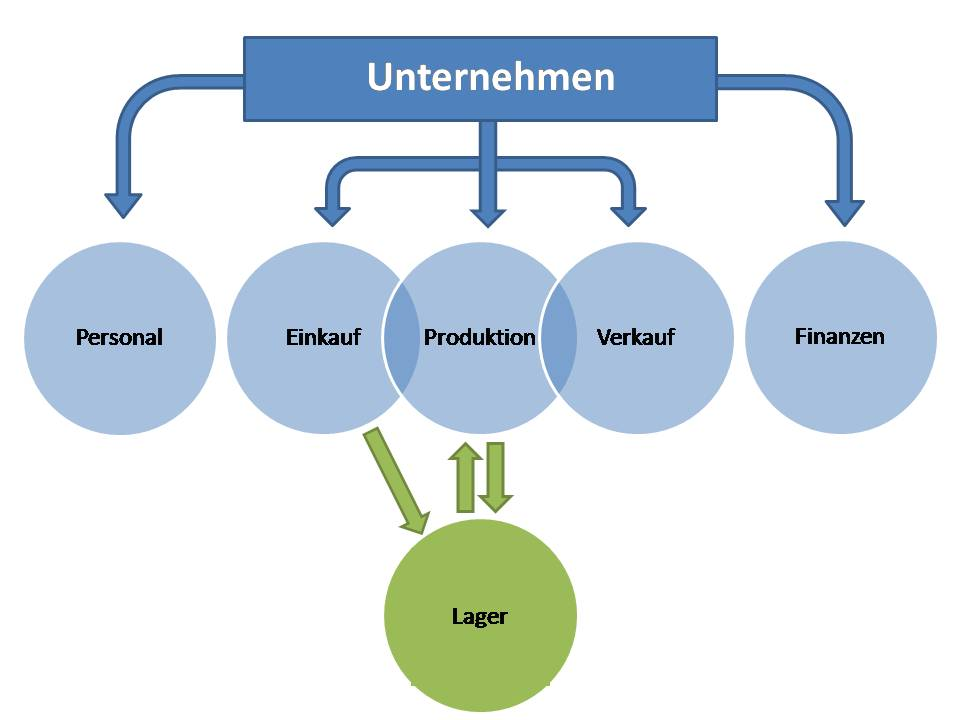
\includegraphics[width=0.75\textwidth]{20_Spielwelt/20_Unternehmen/Unternehmensstruktur.jpg}
\caption{Unternehmensstruktur}
\end{figure}

Im Einkauf werden die zur Produktion benötigten Bauteile zu den aktuellen Bauteilpreisen eingekauft und auf Lager gelegt, sodass dann anhand des Lagerbestandes in der Produktion festgelegt werden kann, wie viele Raumschiffe von den einzelnen Typen hergestellt werden. Es liegen keine Mindest- und Höchstmengen vor, sodass der Spieler hier beliebig variieren kann. Zu beachten sei, dass die gelagerte Menge an Raumschiffen gleich der im Verkauf angebotenen Menge ist. Lediglich auf den Stückpreis kann im Verkauf Einfluss genommen werden. Ob das Angebot zu dem festgelegten Preis voll abgesetzt werden kann, bestimmt die Nachfrage auf dem Markt und das Verhalten der Konkurrenzunternehmen. Diejenigen Raumschiffe, die während der aktuellen Runde nicht abgesetzt werden konnten, verbleiben im Lager. 
\\
\\
Für die Organisation und Verwaltung des Lagers wurden zwei Varianten analysiert. Die erste Variante beschreibt im Wesentlichen  ein Lager, wie man es in der Realität auch vorfinden würde. Die Lagergröße und damit die Kapazität, Bauteile und Raumschiffe zu lagern und damit auch zu produzieren, sind beschränkt. Pro Runde fallen fixe Kosten an, unabhängig davon, wie stark das Lager ausgelastet ist. Bei einem mittelgroßen Lager und geringer Auslastung, z.B. in der Anfangszeit des Unternehmens, stellt es eine enorme finanzielle Belastung dar. Wählt man das Lager von Anfang an eher klein, so sind die anfänglichen Fixkosten zwar geringer, bei einer Produktionserhöhung fallen aber schnell - schneller als bei einem anfänglichen großen Lager - Sprungfixkosten durch die Zusatzinvestitionen des Anbaus oder Kaufs einer neuen Lagerhalle an. 
\\
Variante B beschreibt eine Art dynamisches Lager, in dem man die Problematik der Fixkosten umgeht, in dem allein variable Kosten pro eingelagertem Bauteil oder Raumschiff anfallen (vgl. Datenbasis). Die Größe des Lagers kennt keine Kapazitätsgrenze, sodass jederzeit Objekte eingelagert werden können. Konkret heißt das, dass bei einem leeren Lager keine Kosten für das Unternehmen anfallen. Geplant, aber zu diesem Zeitpunkt noch nicht umgesetzt, war außerdem, eine Obergrenze für die Kapazitätsgrenze einzuführen, die durch Zusatzinvestitionen erweitert werden kann, um einen zusätzlichen Parameter zu gewinnen, der die Ausbringungsmenge kontrolliert. 
\\
\\
Eine weitere Besonderheit kann sich in der Produktion durch niedrig qualifiziertes Personal ergeben. Je geringer die Qualitätsstufe einer Arbeitskraft ist, d.h. je höher der Anteil der R2D2 und Kampfdroiden im Verhältnis zum Anteil der Droidekas sind, desto größer ist die Wahrscheinlichkeit, dass bei der Produktion eines Raumschiffs Ausschuss entsteht (vgl. Datenbasis - Personal). In diesem Falle kann auf zwei Arten reagiert werden. Zum einen kann die Personalabteilung ihre Droiden aufrüsten, um vorbeugend in eine zuverlässige Fertigung der Raumschiffe zu investieren. Zum anderen ist es dem Unternehmen auch möglich, bei angefallenem Ausschuss für die mangelhaften Raumschiffe Zusatzinvestitionen zu leisten, um diese doch noch marktfähig zu machen und schließlich zu verkaufen. Die hohe Bedeutung dieses Punktes wird klarer, wenn man bedenkt, dass ein Unternehmen gerade in seiner Anfangsphase bedingt durch wenige zur Verfügung stehende Ressourcen nur eine vergleichsweise geringe Zahl an Raumschiffen produzieren und absetzten kann. An dieser Stelle muss es Möglichkeiten geben, die eventuell anfallenden, mangelhaften Raumschiffe durch einen in Relation stehenden Aufwand an den Markt zu bringen. Ist diese Option nicht gegeben, so hätte das Unternehmen keine Chance, sich eine Stellung auf dem Oligopolmarkt zu verschaffen und würde an seinen hohen Anfangseinbußen durch den Totalverlust des Ausschusses zu Grunde gehen. 
\\
\\
In diesem Zusammenhang wird auch die Notwendigkeit gewiss, das Konto des Unternehmens, das über die Finanzabteilung verwaltet wird, zu einem festen Zinssatz überziehen zu können. Hier war anfänglich die Überlegung, genau diese Funktion nicht aufzunehmen. Ein Unternehmen könnte so nur diejenigen finanziellen Tätigkeiten durchführen, für die genügend Kapital vorhanden ist, also möglicherweise die oben angesprochenen Zusatzinvestitionen nicht leisten. Aus diesem Grund wurde im Laufe der Bearbeitung hier eine Änderung vorgenommen.  Neben diesem Argument, spricht auch die Tatsache, dass hierdurch risikoreiche Entscheidungen und Aktionen des Unternehmens durchführbar sind, für die Kontoüberziehung.

\autorende{}
